\chapter{Additional plots and tables} \label{appB:additional}

%%%%%%%%%%%%%%%%%%%%%%%%%%%%%%%%%%%%%%%%%%%%%%%%%%%%%%%%%%%%%%%%%%%%%%%
%%%%%%%%%%%%%%%%%%%%%%%%%%%%%%%%%%%%%%%%%%%%%%%%%%%%%%%%%%%%%%%%%%%%%%%

\section{Chapter 3: Bayesian estimation} \label{appB1:chapter3}

\subsection{To center or not to center} \label{appB1:noncenter}
%
\begin{figure}[!h]
	\centering
	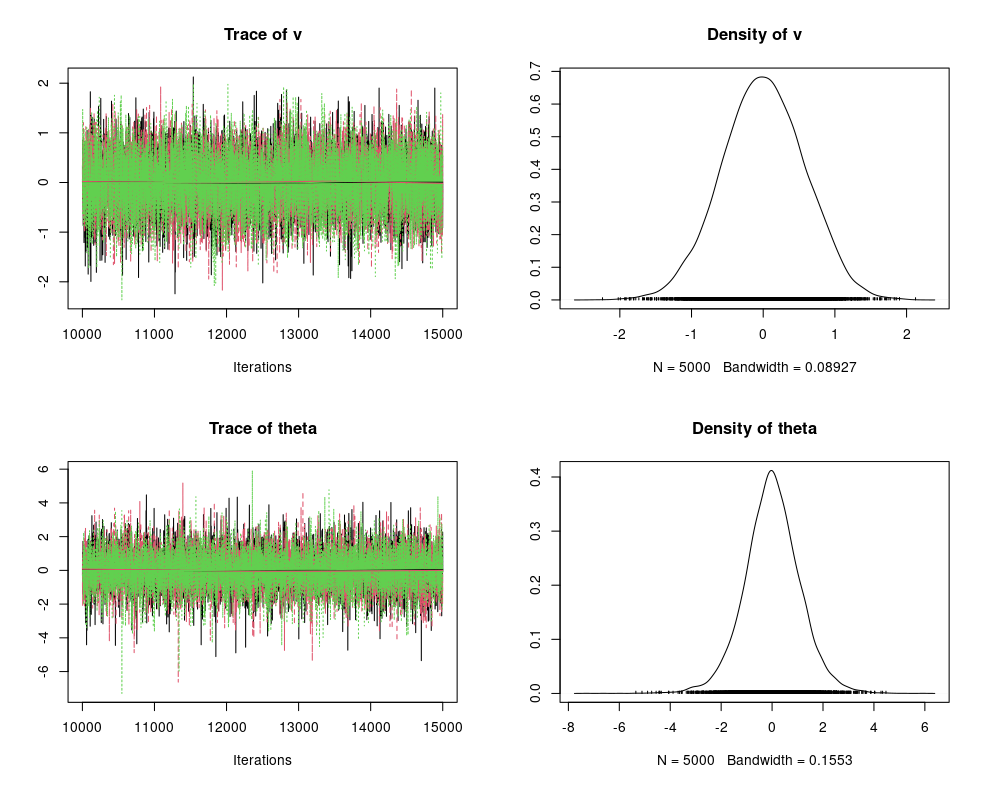
\includegraphics[width=0.8\linewidth]{1_jags_CE_simple}
	%
	\caption[The Devil's funnel. Centered Parametrization. JAGS]%
	{The Devil's funnel. Centered Parametrization implemented in JAGS. It shows the traceplot and distribution of the parameters of interest.}
	\label{fig:devil_CE_simple_jags}
\end{figure}
%
\begin{figure}[!h]
	\centering
	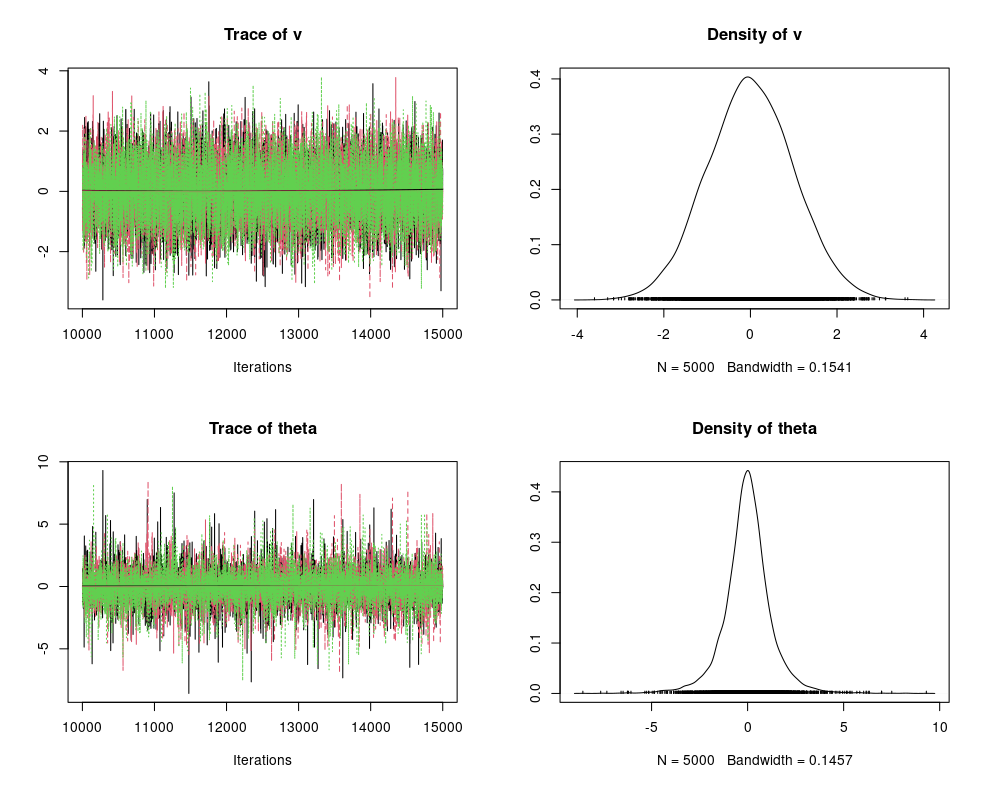
\includegraphics[width=0.8\linewidth]{2_jags_CE_priors}
	%
	\caption[The Devil's funnel. Centered Parametrization with mildly informative priors. JAGS]%
	{The Devil's funnel. Centered Parametrization with mildly informative priors implemented in JAGS. It shows the traceplot and distribution of the parameters of interest.}
	\label{fig:devil_CE_prior_jags}
\end{figure}
%
\begin{figure}[!h]
	\centering
	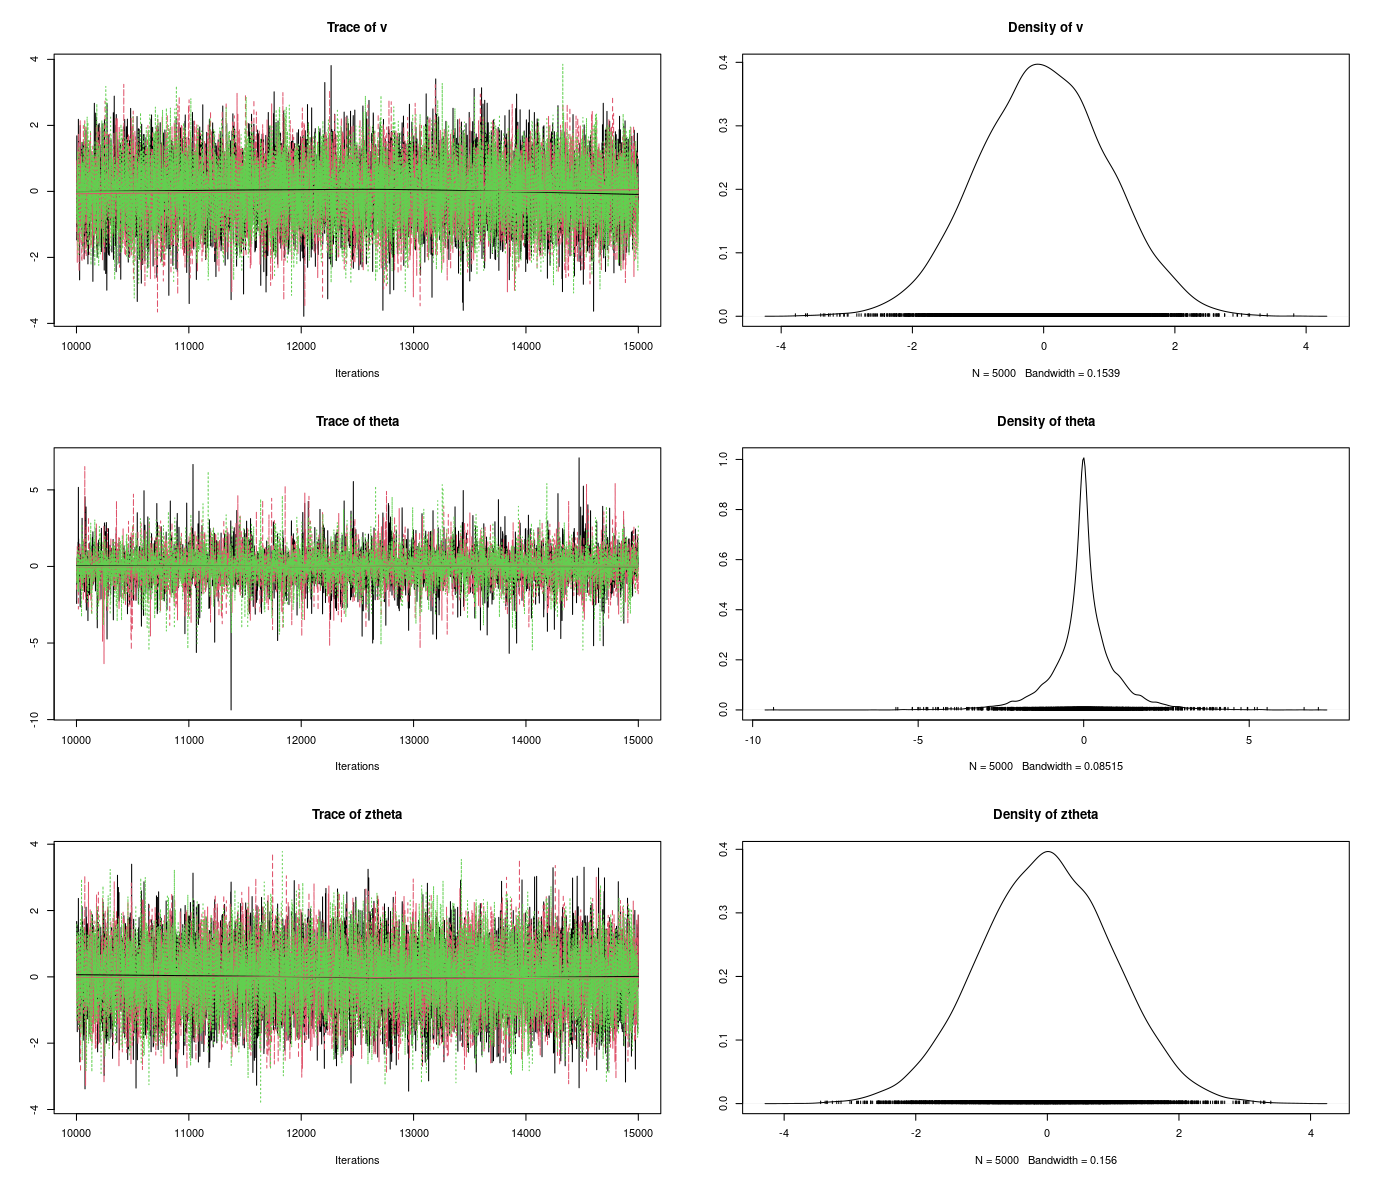
\includegraphics[width=0.8\linewidth]{3_jags_NC}
	%
	\caption[The Devil's funnel. Non-Centered Parametrization. JAGS]%
	{The Devil's funnel. Non-Centered Parametrization implemented in JAGS. It shows the traceplot and distribution of the parameters of interest.}
	\label{fig:devil_CE_NC_jags}
\end{figure}

%%%%%%%%%%%%%%%%%%%%%%%%%%%%%%%%%%%%%%%%%%%%%%%%%%%%%%%%%%%%%%%%%%%%%%%


%%%%%%%%%%%%%%%%%%%%%%%%%%%%%%%%%%%%%%%%%%%%%%%%%%%%%%%%%%%%%%%%%%%%%%%
%%%%%%%%%%%%%%%%%%%%%%%%%%%%%%%%%%%%%%%%%%%%%%%%%%%%%%%%%%%%%%%%%%%%%%%


\section{Chapter 4: Simulation study} \label{appB2:chapter4}

Trace, trank and ACF plots for all models, parametrizations, and replicas can be found in the images section of the accompanying github page:

\url{https://github.com/jriveraespejo/thesis/tree/master/images/chains}

